\begin{surferPage}[7-gon]{A 7-gon-symmetric Septic}
    %This surface which looks like a star has degree $7$. 
		Ova ploha koja izgleda poput zvijezde ima stupanj $7$.
    %Until recently its number of singularities, $84$, was still the
		Do nedavno je broj njenih singulariteta, $84$, bio 
    %maximum number of real singularities known for septics;
		najve\'{c}i poznati broj realnih singulariteta za septike;
    %only in 2004, Oliver Labs improved this world record to $99$.
		tek je 2004. Oliver Labs pove\'{c}ao svjetski rekord na $99$.
  
  
 %The three cushions which one can see in the interactive picture, 
Tri jastuka koja mo\v{z}emo vidjeti na interaktivnoj slici
    %are caused by the use of Chebychev polynomials, similar to the Chmutov
    %Octic. 
		uzrokovana su upotrebom Chebychevljevih polinoma, sli\v{c}no Chmutovoj Oktici.
    %In fact, this star shaped surface is another variant of Chmutov's surfaces.
		U stvari, ova ploha u obliku zvijezde je varijanta Chmutove plohe.
    %Here, the plane curve $T_d(x)+T_d(y)$ was replaced by a regular $7$-gon
		Ovdje je ravninska krivulja $T_d(x)+T_d(y)$ zamjenjena pravilnim sedmerokutom
    $S_7(x,y)$: 
   \[S_7(x,y) + \lambda \cdot T_d(z) = 0,\]
    %for a suitably chosen 
		za prikladno izabrani $\lambda\in\RR$. 
    \vspace*{-0.3em}
    \begin{center}
      \begin{tabular}{c@{\qquad}c}
        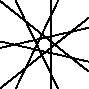
\includegraphics[height=1.5cm]{./../../common/images/labsseptic1.pdf}
        &
        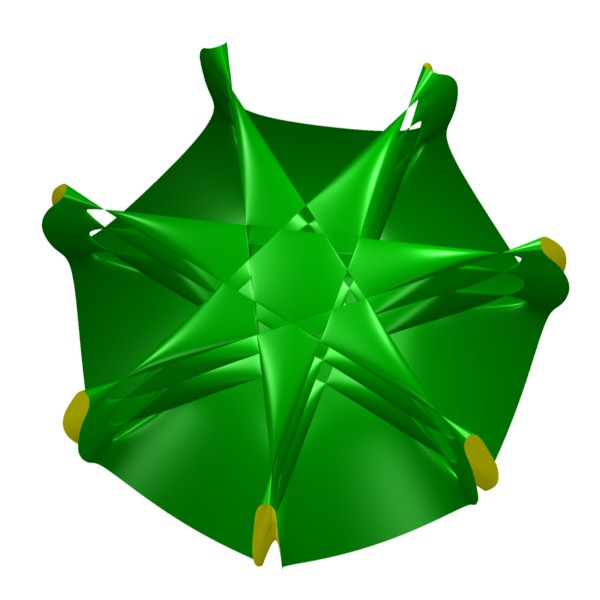
\includegraphics[height=1.5cm]{./../../common/images/septic_7eck_von_oben}
      \end{tabular}
    \end{center}
    \vspace*{-0.3em}   
   %This variant of Chmutov's construction is provided by Duco van Straten.
	Ovu varijantu Chmutove konstrukcije omogu\'{c}io je Duco van Straten.
\end{surferPage}
